\section{含噪评价}
\label{sec:rs-noise}

到目前为止，读数都等于真实代价。如果每次评价带有噪声，如式~\eqref{eq:rs-reading}，同一个候选评价两次也会得到不同的数。噪声影响了算法的哪些环节，最好记录的含义变成了什么，额外的评价应当花在哪里？

\paragraph{噪声影响三个环节}
先明确优化的对象。本节设读数误差$\varepsilon$的均值为零，要最小化的是期望代价$f(\bm{x})=\mathbb{E}[\tilde f(\bm{x})]$；如果关心的是分位数或最坏情形，要先改定目标。这也说明，第~\ref{sec:rs-sa-barrier}节的定理和第~\ref{sec:rs-es-selection}节的单调性都是针对精确代价的，不能直接用到含噪读数上。

第一个受影响的是\textbf{接受}。设真实上坡量为$2$，$T=0.5$，无噪声时接受概率为$\mathrm{e}^{-4}\approx0.018$。若两次读数的误差各自服从$\mathcal{N}(0,1)$，接受概率的平均值变成约$0.157$，是原来的八倍多。噪声的效果相当于抬高了温度。

第二个是\textbf{排序}：种群中的名次可能和真实好坏相反，选择压力被噪声稀释。第三个是\textbf{最好记录}，这是最隐蔽的，下面专门讨论。

\paragraph{最低读数偏向有利噪声}
设有$N$个候选，真实代价都是$0$，读数相互独立，服从$\mathcal{N}(0,1)$。算法把读数最低的那个当作最好解，它的读数是$N$个标准正态变量的最小值，期望是负的。

$N=2$时可以手算。由$\min(a,b)=\tfrac12(a+b-\lvert a-b\rvert)$，两个读数$Z_1,Z_2$的最小值的期望是
\[
 \mathbb{E}\min(Z_1,Z_2)=-\tfrac12\mathbb{E}\lvert Z_1-Z_2\rvert.
\]

$Z_1-Z_2\sim\mathcal{N}(0,2)$，$\mathbb{E}\lvert Z\rvert=\sqrt{2/\pi}$，于是
\[
 \mathbb{E}\min(Z_1,Z_2)=-\tfrac12\cdot\sqrt2\cdot\sqrt{\frac2\pi}=-\frac{1}{\sqrt\pi}\approx-0.564.
\]

$N$增大，这个偏差继续变大。图~\ref{fig:rs-noise-selection}(a)显示$N=1000$时最低读数的均值约为$-3.24$，虽然所有候选的真实代价都是$0$。比较的次数越多，“最好”的读数越乐观。

\begin{BookInlineFigure}
 \centering
 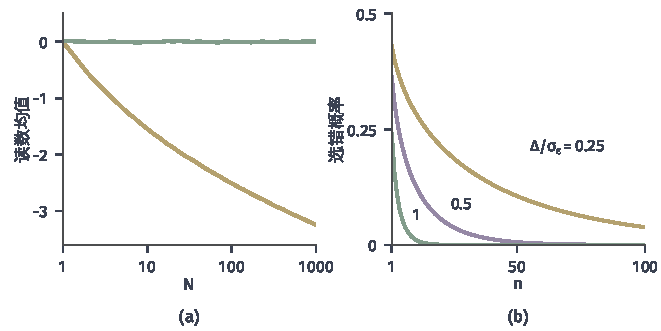
\includegraphics[width=112mm]{figures/05-optimization/05-stochastic-optimization/matplotlib/rs-noise-selection/figure.pdf}
 \caption{噪声下的选择。(a)$N$个真实代价都为$0$的候选，噪声服从$\mathcal{N}(0,1)$，黄线是最低读数的均值，绿线是对选出者重新读一次的均值，由$20000$次抽样估计。(b)两候选真实差为$\Delta$，噪声标准差为$\sigma_\varepsilon$，各读$n$次后按样本均值选错的概率，按式~\eqref{eq:rs-wrong-selection}计算。}
 \label{fig:rs-noise-selection}
\end{BookInlineFigure}

\subsection{候选比较}
\label{sec:rs-noise-compare}

两个候选的读数不同，这个差别是真的吗？这一小节讨论要读多少次才能下判断，以及读数应当分给谁。

\paragraph{重复读数}
设候选$\bm{a}$的真实代价比$\bm{b}$低$\Delta>0$。每个候选独立读$n$次，取样本均值。读数的噪声方差都是$\sigma_\varepsilon^2$时，样本均值之差的方差是$2\sigma_\varepsilon^2/n$。

样本均值之差的标准差按$1/\sqrt{n}$下降，而要分辨的真实差$\Delta$不变，所以$\Delta$越小，需要的读数越多。

\begin{theorem}[两候选比较的错误概率]
\label{thm:rs-comparison}
设两候选的读数相互独立，方差都是$\sigma_\varepsilon^2$，真实代价差为$\Delta>0$，各读$n$次后选样本均值较低者。若噪声服从高斯分布，选错的概率为
\begin{equation}
 \mathbb{P}(\text{选错})=\Phi\Bigl(-\frac{\Delta}{\sigma_\varepsilon}\sqrt{\frac{n}{2}}\Bigr),
 \label{eq:rs-wrong-selection}
\end{equation}
其中$\Phi$是标准正态分布函数。若只假定方差有限，则有
\begin{equation}
 \mathbb{P}(\text{选错})\leq\frac{2\sigma_\varepsilon^2}{n\Delta^2}.
 \label{eq:rs-wrong-chebyshev}
\end{equation}
\end{theorem}

\begin{proof}
记$\bar{a},\bar{b}$为两个样本均值，令$W=\bar{a}-\bar{b}+\Delta$，$W$的均值为$0$，方差为$2\sigma_\varepsilon^2/n$。选错即$\bar{a}\geq\bar{b}$，也就是$W\geq\Delta$。

高斯情形下$W\sim\mathcal{N}(0,2\sigma_\varepsilon^2/n)$，标准化后即得式~\eqref{eq:rs-wrong-selection}。方差有限时，由Chebyshev不等式，
\[
 \mathbb{P}(W\geq\Delta)\leq\mathbb{P}(\lvert W\rvert\geq\Delta)\leq\frac{2\sigma_\varepsilon^2}{n\Delta^2}.
\]
\end{proof}

图~\ref{fig:rs-noise-selection}(b)是式~\eqref{eq:rs-wrong-selection}。$\Delta/\sigma_\varepsilon=1$时，一次读数选错的概率约为$0.24$，$n=4$时约为$0.079$，$n=16$时约为$0.002$。$\Delta/\sigma_\varepsilon=0.5$时要$n=16$才降到$0.079$，差减半，读数要多四倍。这也就是说，$n$按$(\sigma_\varepsilon/\Delta)^2$增长。

方差未知时要用样本方差，置信水平还要计入同时比较的次数，这些统计保证的条件和推导可参考\BookChapterRef{chap:finite-sample-error-bounds}{卷八第4章“有限样本的误差上界”}。

\paragraph{把预算分给难分辨的候选}
候选的差别悬殊时，一两次读数就够分辨；差别小的，才值得多读。因此比全体平均分配读数更省的安排是：先给每个候选少量读数，计算均值和不确定性区间，淘汰区间明显落后的候选，把后续读数分给仍难分辨的那些。

这里要区分两种错误。比较误差是已见候选之间排错了名次；覆盖不足是更好的点根本没被评价过。多读几次已见的候选，只能减少前者。复核已见候选不能证明不存在更优的未见点。用于复核的读数和探索新候选竞争同一份预算，两者的分配要依问题决定。

\subsection{历史最好解的复核}
\label{sec:rs-noise-reeval}

上面看到最低读数偏向有利噪声。这一小节的问题是：对选出来的候选还能相信什么，要怎样复核？

\paragraph{选中之后重新评价}
式~\eqref{eq:rs-best-record}的记录是一次选择的结果，所以这个读数带偏。对选出的候选\textbf{用新的独立读数}重新评价，得到的就是无偏的估计。

原因是：选择只依赖旧的读数，新的噪声与选择无关。设选中的候选是$\hat{\bm{x}}$，给定$\hat{\bm{x}}$的条件下，新读数的条件期望是$f(\hat{\bm{x}})$，所以
\begin{equation}
 \mathbb{E}\bigl[\tilde f_{\mathrm{new}}(\hat{\bm{x}})\mid\hat{\bm{x}}\bigr]=f(\hat{\bm{x}}).
 \label{eq:rs-fresh-reading}
\end{equation}
图~\ref{fig:rs-noise-selection}(a)的绿线正是这一点，重新读一次的均值稳定在真实值$0$附近。

条件是新读数必须与用于选择的读数独立。把旧读数和新读数平均，偏差只是减小，并不消失。若一批复核读数又用来在多个候选中再选一次，新的选择偏差又产生了，要再留一批读数来做最终的估计。

\paragraph{新旧记录的比较}
旧记录的读数是经过多次比较选出来的最小值，新候选只有一次读数，两者并不能等量比较。$(1+1)$策略一旦遇到一次特别幸运的读数，后代的一次读数几乎都比不过它，这个亲代就长期占位，算法看起来“收敛”了，实际只是被一次噪声卡住。

常用的修正是每一代重新评价亲代，或者让记录中的候选累积多次读数后再参与比较。这些额外的评价都要计入预算，代价是每代评价数增加。

\paragraph{要记录什么}
搜索过程实际使用的选解规则要原样记录：是取最低的单次读数，还是取重复读数的最低均值，还是另留一批独立读数做最后的裁决。

报告结果时也要说清每个数字的来源。“最好值”如果是搜索过程中的最低读数，就是偏乐观的；如果来自独立的复核读数，才能作为对$f(\hat{\bm{x}})$的估计。样本复用省评价次数，但信息依赖也要一并交代。
